
\chapter{Results}
% LC 25pgs
\label{Results} 

%This chapter presents the outputs that you produced, by applying the methods that you have selected, including e.g. analysis, design, prototyping, experimental work, evaluation, etc.  
  
%How you report these results will depend on the nature of the work. It may be helpful to divide them into basic data (e.g., for a project that developed a software product, requirements specification, test data, etc.) and analysis of the data (e.g. statistical analyses, evaluation analyses, etc.). Remember that you are informing the reader of what you have produced and found and emphasising the interesting parts, so summarising at the end of each major section is useful.  
  
%It is usually very helpful for the readers to include graphics and diagrams, for instance to clarify software design or requirements, identify key trends and relationships in empirical data, etc. If you do so, be sure to refer to these figures in the text and use them as evidence to support what you are explaining or arguing; and be sure that your figures are well designed and clearly presented – do not just use default settings of the software you are using in producing them.  
  
%It is essential that you identify clearly what you accomplished or produced yourself, as opposed to what existed before you started your individual project or was provided by others. For instance, some projects build new software on top of an existing code base, add new data to an existing body of data, or are executed by a student as a member of a team. It is essential to indicate what parts of the activities and results which you report are your own work. If this is left unclear, the markers are instructed not to give credit for work that they cannot attribute to you. Ambiguity would attract penalties for poor academic practice, with delays caused by any investigation (deception would be treated as academic misconduct, of course, which may lead to expulsion).

%-----------------------------------
%	Network training
%-----------------------------------



\section{Network training and simulator testing}
\label{results:net-training} 
% write up, label runs and make reference
The first working model (able to successfully self-drive around the Generated Track) was   20201107210627\_nvidia1.h5. A video was generated using the recording screen utility Kazam (\cite{Kazam2020}), recording at 15fps (frames per second), and published at  \href{https://youtu.be/9z0mMtOnUUc}{https://youtu.be/9z0mMtOnUUc}. Figure \ref{fig:SimTCPPred}
shows 3 stills from the video containing from left to right, the game engine, the TCP debug output and the prediction engine running.

\begin{figure}[h!]
\centering
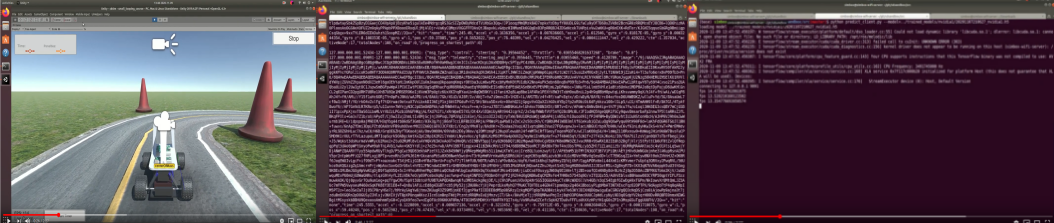
\includegraphics[width=\textwidth]{Figures/SimTCPPred.png}
\caption{Stills of video \href{https://youtu.be/9z0mMtOnUUc}{https://youtu.be/9z0mMtOnUUc} showing left to right: SDSandbox simulated car going around the Generated Track course, TCP Debug (tcpflow) and prediction engine (predict\_ client.py) running}
\label{fig:SimTCPPred}
\end{figure}

The video shows the TCP debugging, prediction engine and the game engine simulated car steering with predictions received over the TCP network. The actual code used to generate the model was not logged at the time the experiment log entry was written in the appendix log (\ref{AppendixD}). By verifying git hash commits (4 commits were made on November 7th) as documented in appendix  a second sanity check model \ref{app_res:36} (20201120171015\_ sanity.h5) was created and found to self-drive successfully around the generated track. A video was made from tcpflow frames as described at the end of \ref{app_res:36}, and uploaded to \href{https://youtu.be/JaSkkh-2xtI}{https://youtu.be/JaSkkh-2xtI}.
The video shows (fps discrepancies considered) that the \ref{app_res:36} model had a better lap around the track.
Model 37 (\ref{app_res:37}) trained with genRoad (including outliers seen in Figure \ref{fig:GeneratedRoadPlusHist}) ) did not do well. The oversteering can be seen in video \href{https://youtu.be/xGDN8qOnv9M}{https://youtu.be/xGDN8qOnv9M}. The steering angle bins and graph plots can be seen in  Figures \ref{fig:tcpflow_20201120184912_bins}  and \ref{fig:tcpflow_20201120184912_graph} in the results appendix.

% a number of runs (e.g. commit 2e5bf1b7 failed prematuraly, most failing to generate a model. Doing a diff on one of them shows that batch size was set to 128
% Could this also be an issue?
% Note in original Alexnet which we assume NVIDIA were using as a design reference, used batch size 128 for TWO channels - TODO write-up in Discussion.

%$ git diff master..2e5bf1b7 train.py | grep batch_size
%-    batch_size = conf.batch_size
%+    batch_size = conf.training_batch_size
%(base) simbox@simbox-wifi-server:~/src(master)$ git diff master..2e5bf1b7 conf.py | grep %batch_size
%+training_batch_size = 128
%-batch_size = 64
%+batch_size = 128 # nvidia1 = 64
%@@ -50,7 +49,5 @@ batch_size = 64
Figure \ref{fig:SkewCleanup} shows from left to right, an overlay of all plots of normalized histogram plots for steering values contained in unity/genRoad directory, the folder containing most outliers (logs\_Thu\_Jul\_ \_9\_16\_00\_15\_2020) and the resulting plot once the outliers' folder was removed from unity/genRoad. 

\begin{figure}[h!]
\centering
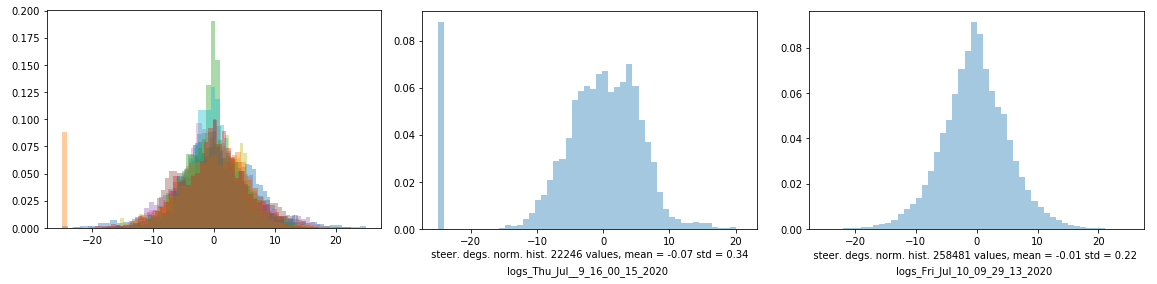
\includegraphics[width=\textwidth]{Figures/SkewCleanup.png}
\caption{Left to right, normalized histograms of all genRoad folders, outlier's folder and all data with outliers removed.}
\label{fig:SkewCleanup}
\end{figure}

Once the outliers were removed, another model was generated with five epochs of training to test if there was any difference in the loss values observed. The resulting model proved useful and was able to drive along the Generated Road course during a few seconds until the simulation was stopped. Below are the normalized histogram and bins recovered from tcplow logs for model  
  
20201120184912\_sanity.h5 referenced in \ref{app_res:37}. The video generated from tcpflow log was uploaded to \href{https://youtu.be/xGDN8qOnv9M}{https://youtu.be/xGDN8qOnv9M}.

\begin{figure}[ht]
 \centering 
 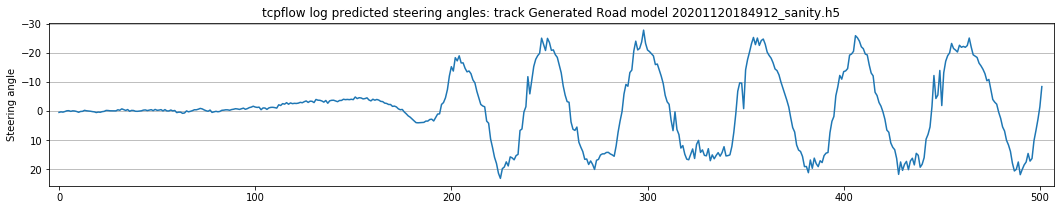
\includegraphics[width=\textwidth]{Figures/tcpflow_20201120184912_sanity_graph.png}
 \caption{Graph of steering angles recovered from tcpflow log genRoad/tcpflow/20201120184912\_sanity\_tcpflow.log for model 20201120184912\_sanity.h5 driving on Generated Road}
 \label{fig:tcpflow_20201120184912_graph}
\end{figure}

\begin{figure}[ht]
 \centering 
 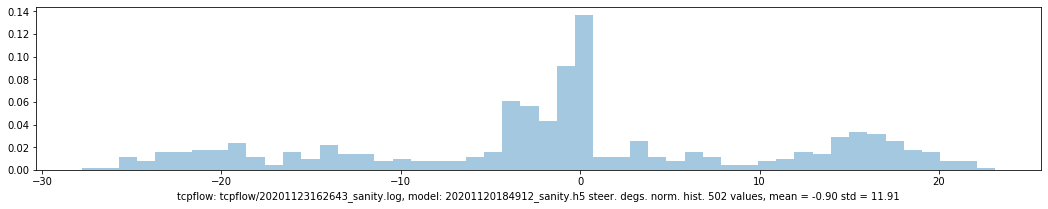
\includegraphics[width=\textwidth]{Figures/tcpflow_20201120184912_sanity_bins.png}
 \caption{Normalized histogram of tcpflow log genRoad/tcpflow/20201120184912\_ sanity \_ tcpflow.log for model 20201120184912\_ sanity.log driving on Generated Road}
 \label{fig:tcpflow_20201120184912_bins} 
\end{figure}

\section{Goodness of steer results}

To compare models, the $G_s$ (Eq. \ref{eq:goodness_of_steer}) was used. Figure  \ref{fig:genTrackOneLap_20201120171015_sanity_gos} contains (discuss):
\begin{itemize}
    \item[--] The PID effect
    \item[--] 
\end{itemize}
The
A second data output was created for the Generated Track circuit. (TODO, create another dataset and plot to compare PID to and manual steering angles).
A video was then created to observe steering angles while recording another dataset on the same lap \href{https://youtu.be/zAmr7a1ImEY}{https://youtu.be/zAmr7a1ImEY}. The video shows steering corrections
% nb recorded at



\begin{figure}[ht]
 \centering 
 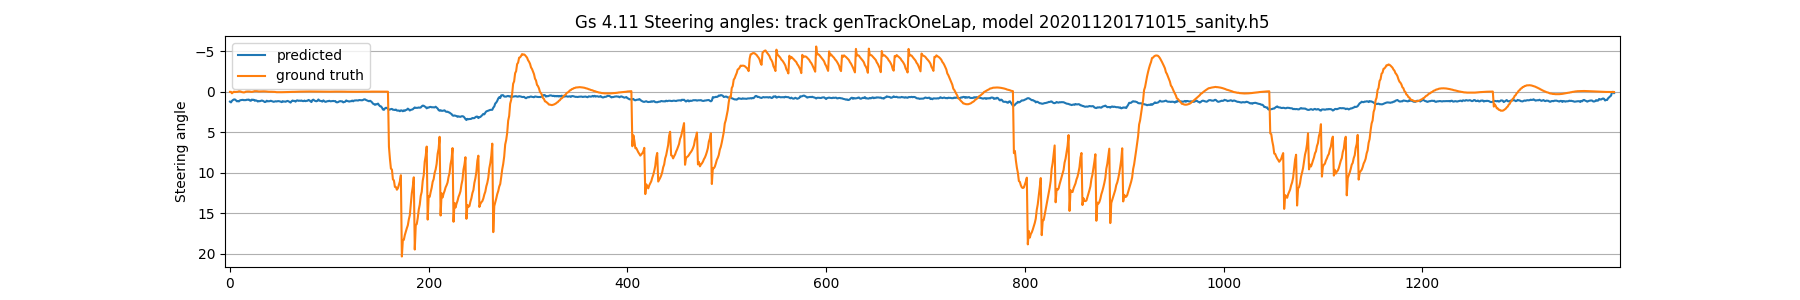
\includegraphics[width=\textwidth]{Figures/sa_genTrackOneLap_20201120171015_sanity.h5.png}
 \caption{Plot containing ground truth steering values recorded in dataset genTrackOneLap .json files and values predicted by model 20201120171015\_ sanity.h5}
 \label{fig:genTrackOneLap_20201120171015_sanity_gos} 
\end{figure}

To confirm the observed acute steering angle variations, a second lap was recorded, producing the same plot
 \label{fig:a_genTrackOneLap_2_20201120171015_sanity} 

\begin{figure}[ht]
 \centering 
 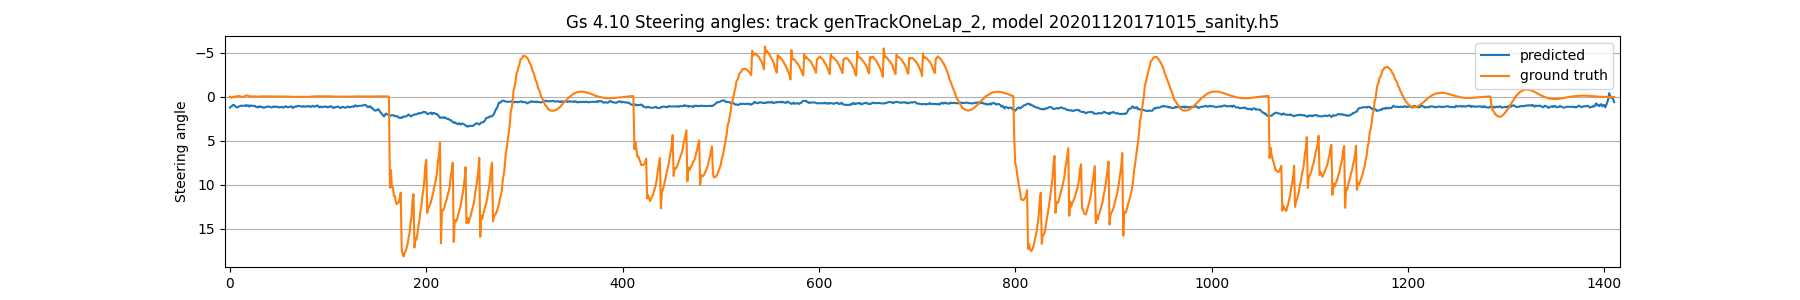
\includegraphics[width=\textwidth]{Figures/sa_genTrackOneLap_2_20201120171015_sanity.h5.png}
 \caption{Plot containing ground truth steering values recorded in dataset genTrackOneLap\_ 2 .json files and values predicted by model 20201120171015\_ sanity.h5, confirming the acute steering angles observed in previous dataset}
 \label{fig:a_genTrackOneLap_2_20201120171015_sanity} 
\end{figure}

The values of Prop and Diff (Proportional and Derivative components of PID steering) were changed while observing steering 
% PID 25, Diff 8, max speed 1.6

This had a smoothing effect to the steering, though the $Gs$ increased:
 \ref{fig:genTrackOneLap_3_20201120171015_sanity_gos} 
 
\begin{figure}[ht]
 \centering 
 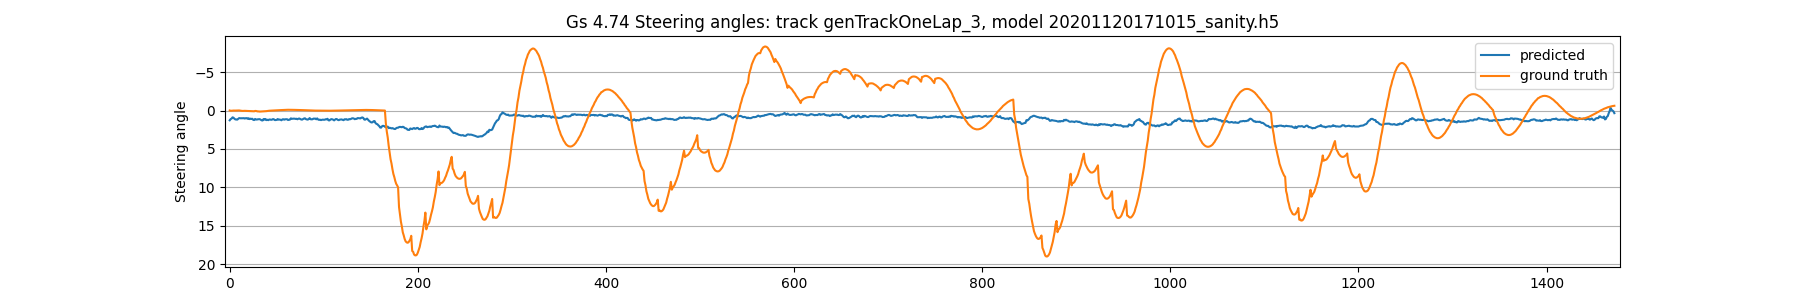
\includegraphics[width=\textwidth]{Figures/sa_genTrackOneLap_3_20201120171015_sanity.h5.png}
 \caption{Plot containing ground truth steering values recorded in dataset genTrackOneLap\_ 3 .json files and values predicted by model 20201120171015\_ sanity.h5, showing the smoothing effect of changing Prop and Diff variables for data capture in Auto w Drive mode}
 \label{fig:genTrackOneLap_3_20201120171015_sanity_gos} 
\end{figure}

We added a video of the model running side by side with network as shown in figure 
\ref{fig:20201120171015_sanity_sim_network}, using a procedure as described in \ref{app_res:41}.

\begin{figure}[ht]
 \centering 
 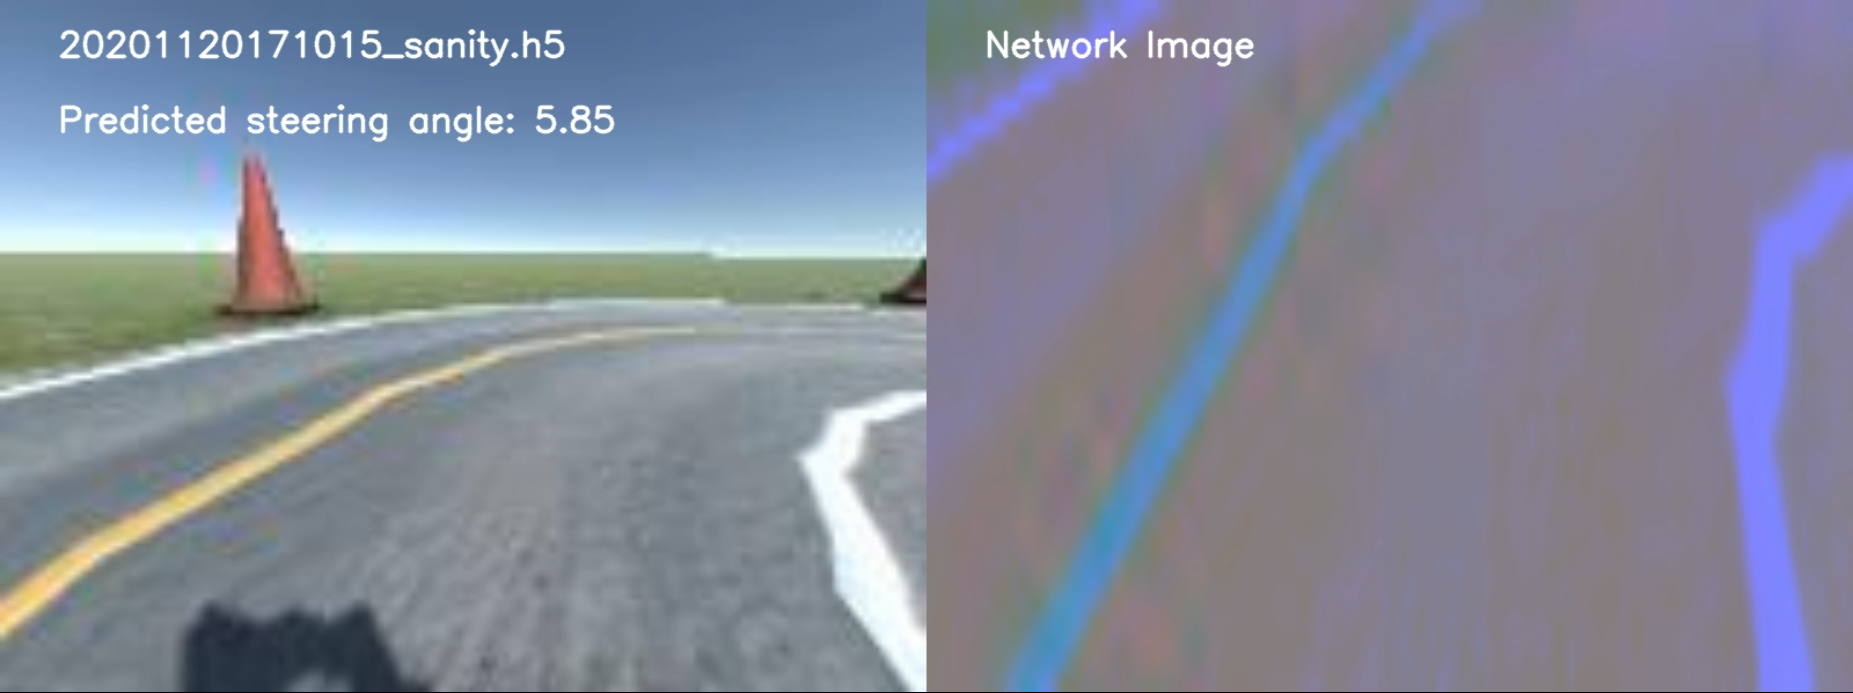
\includegraphics[width=\textwidth]{Figures/20201120171015_sanity_sim_network.png}
 \caption{Video still from \href{https://youtu.be/LEmZJJzJkEE}{https://youtu.be/LEmZJJzJkEE} showing simulator image sent over TCP network on the left with CNN steering angle prediction and processed image (as presented to CNN) on the right}
 \label{fig:20201120171015_sanity_sim_network} 
\end{figure}

\textbf{STOPPED HERE - NEED TO GENERATE STEERING ANGLE PLOT WITH MEAN AND STD} Looks like we might be picking up the simulator steering angle.  \ref{fig:sa_GeneratedTrack_20201120171015_sanity}

\begin{figure}[ht]
 \centering 
 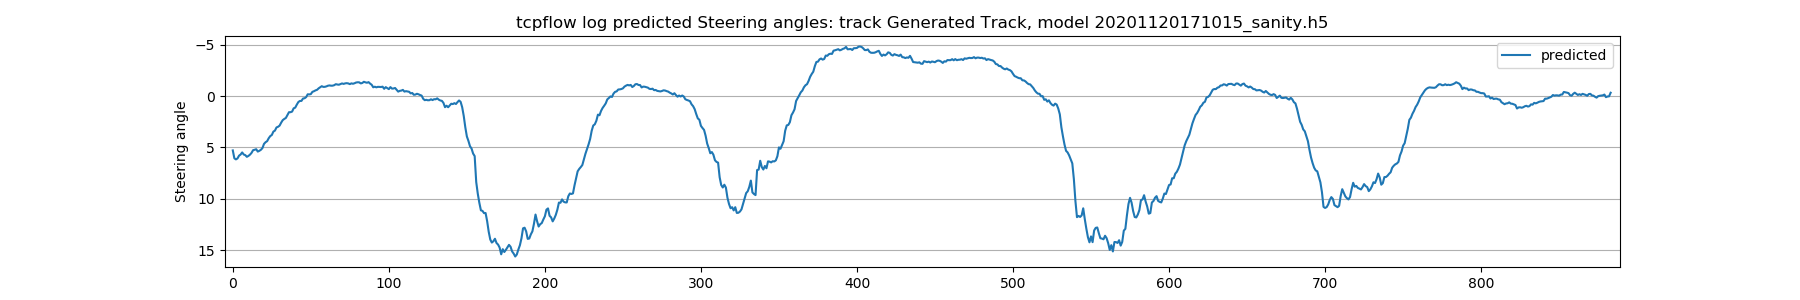
\includegraphics[width=\textwidth]{Figures/sa_GeneratedTrack_20201120171015_sanity.h5.png}
 \caption{Video still showing simulator image sent over TCP network on the left with CNN steering angle prediction and processed image (as presented to CNN) on the right}
 \label{fig:sa_GeneratedTrack_20201120171015_sanity} 
\end{figure}
% probably best to more this to results section and reference here
%\begin{verbatim}
%# data: genRoad (log2 renamed)
%# commit: 1ad187d4bff5b6936c065a1aaa15a654ef4d368c
%$ python train.py --model=sanity --outdir=../trained_models
%\end{verbatim}
%this will create the a model in trained\_output/sanity/20201120184912\_sanity.h5
% and run as per procedure described in (TODO add reference).
More results, this time as per run 43 (\ref{app_res:43}) 3 images side by side (Figure 
 \ref{fig:tcpflow_Run43})
 
\begin{figure}[ht]
 \centering 
 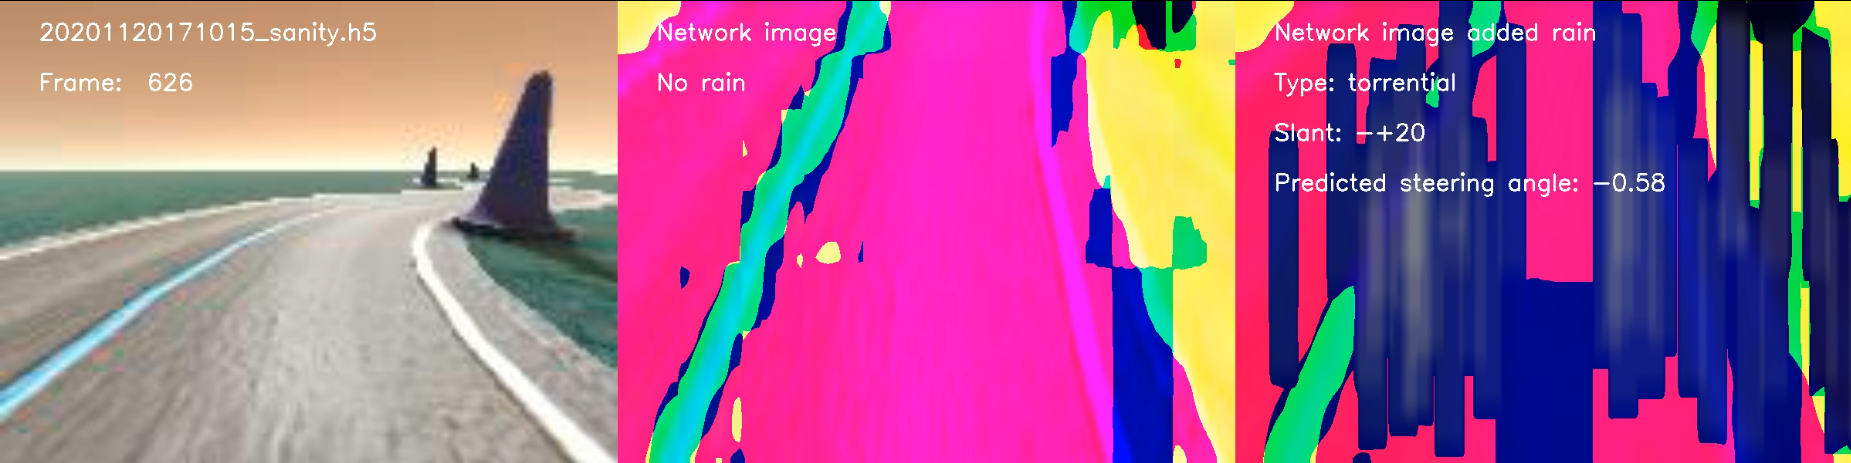
\includegraphics[width=\textwidth]{Figures/tcpflow_Run43.png}
 \caption{Video still TODO add explaination \href{https://youtu.be/57jwwcjbfdE}{https://youtu.be/57jwwcjbfdE}}
 \label{fig:tcpflow_Run43} 
\end{figure}
%\begin{verbatim}
%# data: genRoad (log2 renamed)
%# commit: 1ad187d4bff5b6936c065a1aaa15a654ef4d368c
%$ python train.py --model=sanity --outdir=../trained_models
%\end{verbatim}
%this will create the a model in trained\_output/sanity/20201120184912\_sanity.h5
%and run as per procedure described in (TODO add reference).

\subsection{Modifications to original source codes}
Three libraries used:
\begin{itemize}
    \item SDSandbox
    \item Naoki Augmentation
    \item Automold
\end{itemize}
TODO git diff (in appendix) and itemize modifications.
    
Models are trained with code written in train.py, models.py and conf.py. This code has been modified from the original. To compare changes a git diff can be copying the original code over the source code used in this project and performing a "git diff"
\begin{verbatim}
# clone repository for dissertation
$ git clone https://github.com/dsikar/sdsandbox
# clone original
$ git clone https://github.com/tawnkramer/sdsandbox sandbox_orig
# copy original over dissertation
$ cp sandbox_org/src/* sdsandbox/src
# compare
$ cd sdsandbox 
$ git diff
\end{verbatim}


Starting with the NVIDIA baseline, a number of hyperparameters were trialed. The initial setup failed to generate usable models. 
The table below presents training results for best trained models.

% training with one parameter

\section{Simulated self-driving car}

Using the baseline neural network architecture as described in 
Models trained with no image pre-processing, did not perform well, leading to cars driving off the road, as shown in Fig.  sequence.

% data gathered on Robot Racing League track
We gathered 10 laps of data on the Robot Racing League track, with maximum speed set to 2.1, proportional control set to 16 and differential set to 77. Maximum steer was set to 25 (degrees). Corresponding to 12778 .jpg image files and the same number of  .json files, containing corresponding throttle and steering angle values recorded at the moment image was saved by simulator. This can be seen in the calls to Update() and SaveCamSensor functions in  
\begin{verbatim}
./Assets/Scripts/Logger.cs
\end{verbatim}

\section{Generated Track performance}


The $G_s$ (goodness-of-steer) model performance score, was obtained by recording one full lap and comparing steering angles with model predictions.

\section{Datasets}

The following training datasets were generated:

Origin  Directory   Number of files Comment
SDSandbox   unity/smallLoopingCourse/log/* 34443 from small\_looping\_course
SDSandbox   unity/warehouse/*   41126 From Warehouse course
SDSandbox   unity/smallLoop/*   45422   From small\_looping\_course
SDSandbox   unity/roboRacingLeague/* 12778 From "Robot Racing League" course
SDSandbox   unity/log\_sample   25791   From small\_looping\_course
SDSandbox   unity/genRoad 280727 From "Generated Road" course



Following the list of data deliverables (\ref{Deliverables-Datasets}) the Udacity data consisting of two files 

\subsection{Locating rainy sections with Mechanical Turk}
For Mechanical Turk, the data that looked most promising was Ford V2 Log 1 and V3 Log 1, both described as "freeway, overpass, bridge, cloudy". We drew 50 images uniformly from each log and added 5 images with rain that were expected to be labelled as such. The 105 images were then added to a SageMaker Ground Truth job. The platform works as a wrapper around Mechanical Turk as it facilitates the creation of user interfaces (Figure \ref{fig:MechTurkCreateJob})
% rainy files created with automold/RainyImagesDissertationPlot.ipynb
\begin{figure}[h!]
\centering
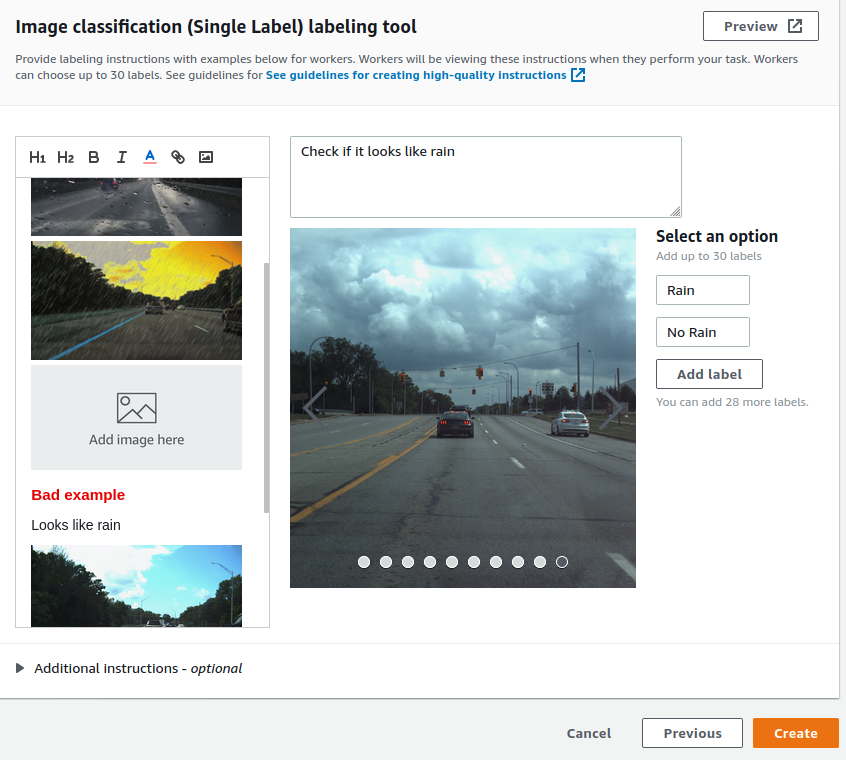
\includegraphics[width=10cm]{Figures/MechTurkCreateJob.png}
\caption{The SageMaker Ground Truth user interface template with two labels ("Rain", "No Rain"), the image to be labeled and examples of correct and incorrect classifications.}
\label{fig:MechTurkCreateJob}
\end{figure}
Labeling tasks are classified as low, medium and high complexity. The prices range from \$0.012 for a low complexity task, with a 5 second estimate to complete, to \$1.20 for a high complexity task with a 3.5 minute estimate to complete.
The task can be configured with an output for time taken by a worker on a single task, the lowest time interval being one minute.
There is also an option to assign more than one worker per dataset object, on account that it can help increase the accuracy of the data labels.
The task was created with the most basic options of one worker, a \$0.012 price per task, a one minute timeout and remained live for 12 hours. 
The images were labelled by Mechanical Turk workers and results made available in a json encoded file (datasets/mechanical-turk/2020-11-21\_22 45 37.json) showing no images had been labeled as "Rain". The assumption then being there are no sections containing rain in the dataset. The Automold library added rain images were also labeled as "No Rain". Figure \ref{fig:MechTurkLabeledImages}
\begin{figure}[h!]
\centering
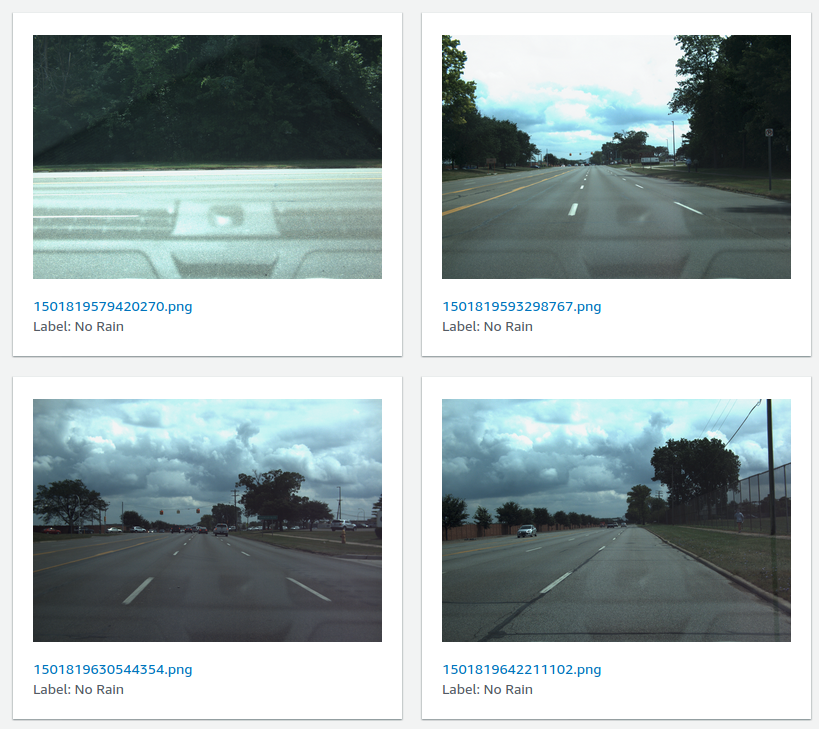
\includegraphics[width=10cm]{Figures/MechTurkLabeledImages.png}
\caption{The SageMaker Ground Truth labeled images detail on Labeling Job Summary page}
\label{fig:MechTurkLabeledImages}
\end{figure}

%-----------------------------------
%	Network running
%-----------------------------------